\documentclass{article}
\usepackage[utf8]{inputenc}
\usepackage[english, russian]{babel}
\usepackage[margin=0.75in]{geometry}
\usepackage{paralist}
\usepackage{amsthm, amsmath, amsfonts, amssymb}
\usepackage{mathtools} % \mathclap
\usepackage{bm}
\usepackage{dsfont}
\usepackage{hyperref}
\usepackage{tabularx}
\usepackage{graphicx}
\usepackage{multirow}
\usepackage{comment}
\usepackage{xcolor, colortbl}
\usepackage{xifthen, xspace}

\title{Домашнее задание №3 по курсу \\ <<Исследование операций>>}
\author{Рак Алексей \\ БГУ}
\date{}

\begin{document}
	
% The list of general commands
\newcommand{\PI}{3.141592654}
\newcommand{\Sum}{\sum\limits}
\newcommand{\Int}{\int\limits}
\newcommand{\Intf}{\int\limits_{-\infty}^{+\infty}}
\newcommand{\Prod}{\prod\limits}
\newcommand{\Max}{\max\limits}
\newcommand{\Min}{\min\limits}
\newcommand{\Var}{\mathbb{V}}
\newcommand{\Exp}{\mathbb{E}}
\newcommand{\ARE}{\mathbb{ARE}}
\newcommand{\argmax}{\arg\max}
\newcommand{\Cov}{\text{Cov}}
\newcommand{\makebold}[1]{\boldsymbol{#1}}
\newcommand{\mean}[1]{\overline{#1}}

% Оценки
\newcommand{\esttheta}{\hat{\theta}}
\newcommand{\estlambda}{\hat{\lambda}}
\newcommand{\estmu}{\hat{\mu}}
\newcommand{\estsigma}{\hat{\sigma}}
\newcommand{\estdelta}{\hat{\delta}}
\newcommand{\estT}{\hat{T}}
\newcommand{\estF}{\hat{F}}
\newcommand{\estC}{\hat{C}}
\newcommand{\estVar}{\hat{\Var}}
\newcommand{\estExp}{\hat{\Exp}}
\newcommand{\estSe}{\hat{\se}}

\newcommand{\tilpsi}{\hat{\psi}}

\newcommand{\mlexi}{\xi_{MLE}}
\newcommand{\mletheta}{\theta_{MLE}}
\newcommand{\mlelambda}{\lambda_{MLE}}
\newcommand{\mlesigma}{\sigma_{MLE}}
\newcommand{\mlepsi}{\psi_{MLE}}

\newcommand{\mmxi}{\xi_{MM}}
\newcommand{\mmtheta}{\theta_{MM}}
\newcommand{\mmlambda}{\lambda_{MM}}
\newcommand{\mmsigma}{\sigma_{MM}}
\newcommand{\mmpsi}{\psi_{MM}}


% Empirical values
\newcommand{\Ecdf}[1]{\estF_n(#1)}
\newcommand{\OPT}{\mathrm{OPT}}
\newcommand{\opt}{\mathrm{opt}}
\newcommand{\boot}{\mathrm{boot}\xspace}
\newcommand{\bias}{\mathrm{bias}\xspace}
\newcommand{\se}{\mathrm{se}\xspace}
\newcommand{\MSE}{\mathrm{MSE}\xspace}
\newcommand{\qm}{\mathrm{qm}\xspace}
\newcommand{\as}{\mathrm{as}\xspace}

\newcommand{\lp}{\left(}
\newcommand{\rp}{\right)}
\newcommand{\lf}{\left\{}
\newcommand{\rf}{\right\}}
\newcommand{\ls}{\left[}
\newcommand{\rs}{\right]}
\newcommand{\lv}{\left|}
\newcommand{\rv}{\right|}


\newcommand{\RR}{\mathbb{R}}
\newcommand{\NN}{\mathbb{N}}
\newcommand{\ZZ}{\mathbb{Z}}

% Классы распределений
\newcommand{\Poisson}{\mathrm{Poisson}\xspace}
\newcommand{\Uniform}{\mathrm{Uniform}\xspace}
\newcommand{\Binomial}{\mathrm{Binomial}\xspace}
\newcommand{\Gammap}{\mathrm{Gamma}\xspace}
\newcommand{\Normal}{\mathcal{N}\xspace}
\newcommand{\LogN}{\mathrm{LogN}\xspace}
\newcommand{\Exponential}{\mathrm{Exp}\xspace}
\newcommand{\Erlang}{\mathrm{Erlang}\xspace}
\newcommand{\Cauchy}{C\xspace}

\newcommand{\boldX}{\boldsymbol{X}}
\newcommand{\boldY}{\boldsymbol{Y}}
\newcommand{\boldx}{\boldsymbol{x}}
\newcommand{\boldy}{\boldsymbol{y}}

% Гипотезы
\newcommand{\RejectRegion}{R}
\newcommand{\pvalue}{\text{p-value}\xspace}


\maketitle

\section*{Матричные игры. Графоаналитический метод.}
\subsection*{10c}
\begin{gather*}\left(\begin{matrix}
2 & 5 & 8 & 11\\
2 & 0 & 9 & 2\\
7 & -3 & -2 & 0\\
 -1 & 5 & 4 & 3\\
\end{matrix}\right)\end{gather*}
Первая стратегия первого игрока доминирует четвертую: $p_4$ = 0; втора стратегия второго игрока доминирует третью и четвертую: $q_3$ = $q_4$ = 0.
\begin{gather*}\left(\begin{matrix}
2 & 5\\
2 & 0\\
7 & -3\\
\end{matrix}\right)\end{gather*}
Первая стратегия первого игрока доминирует вторую $p_2$ = 0, получаем:
\begin{gather*}\left(\begin{matrix}
2 & 5\\
7 & -3\\
\end{matrix}\right)\end{gather*}
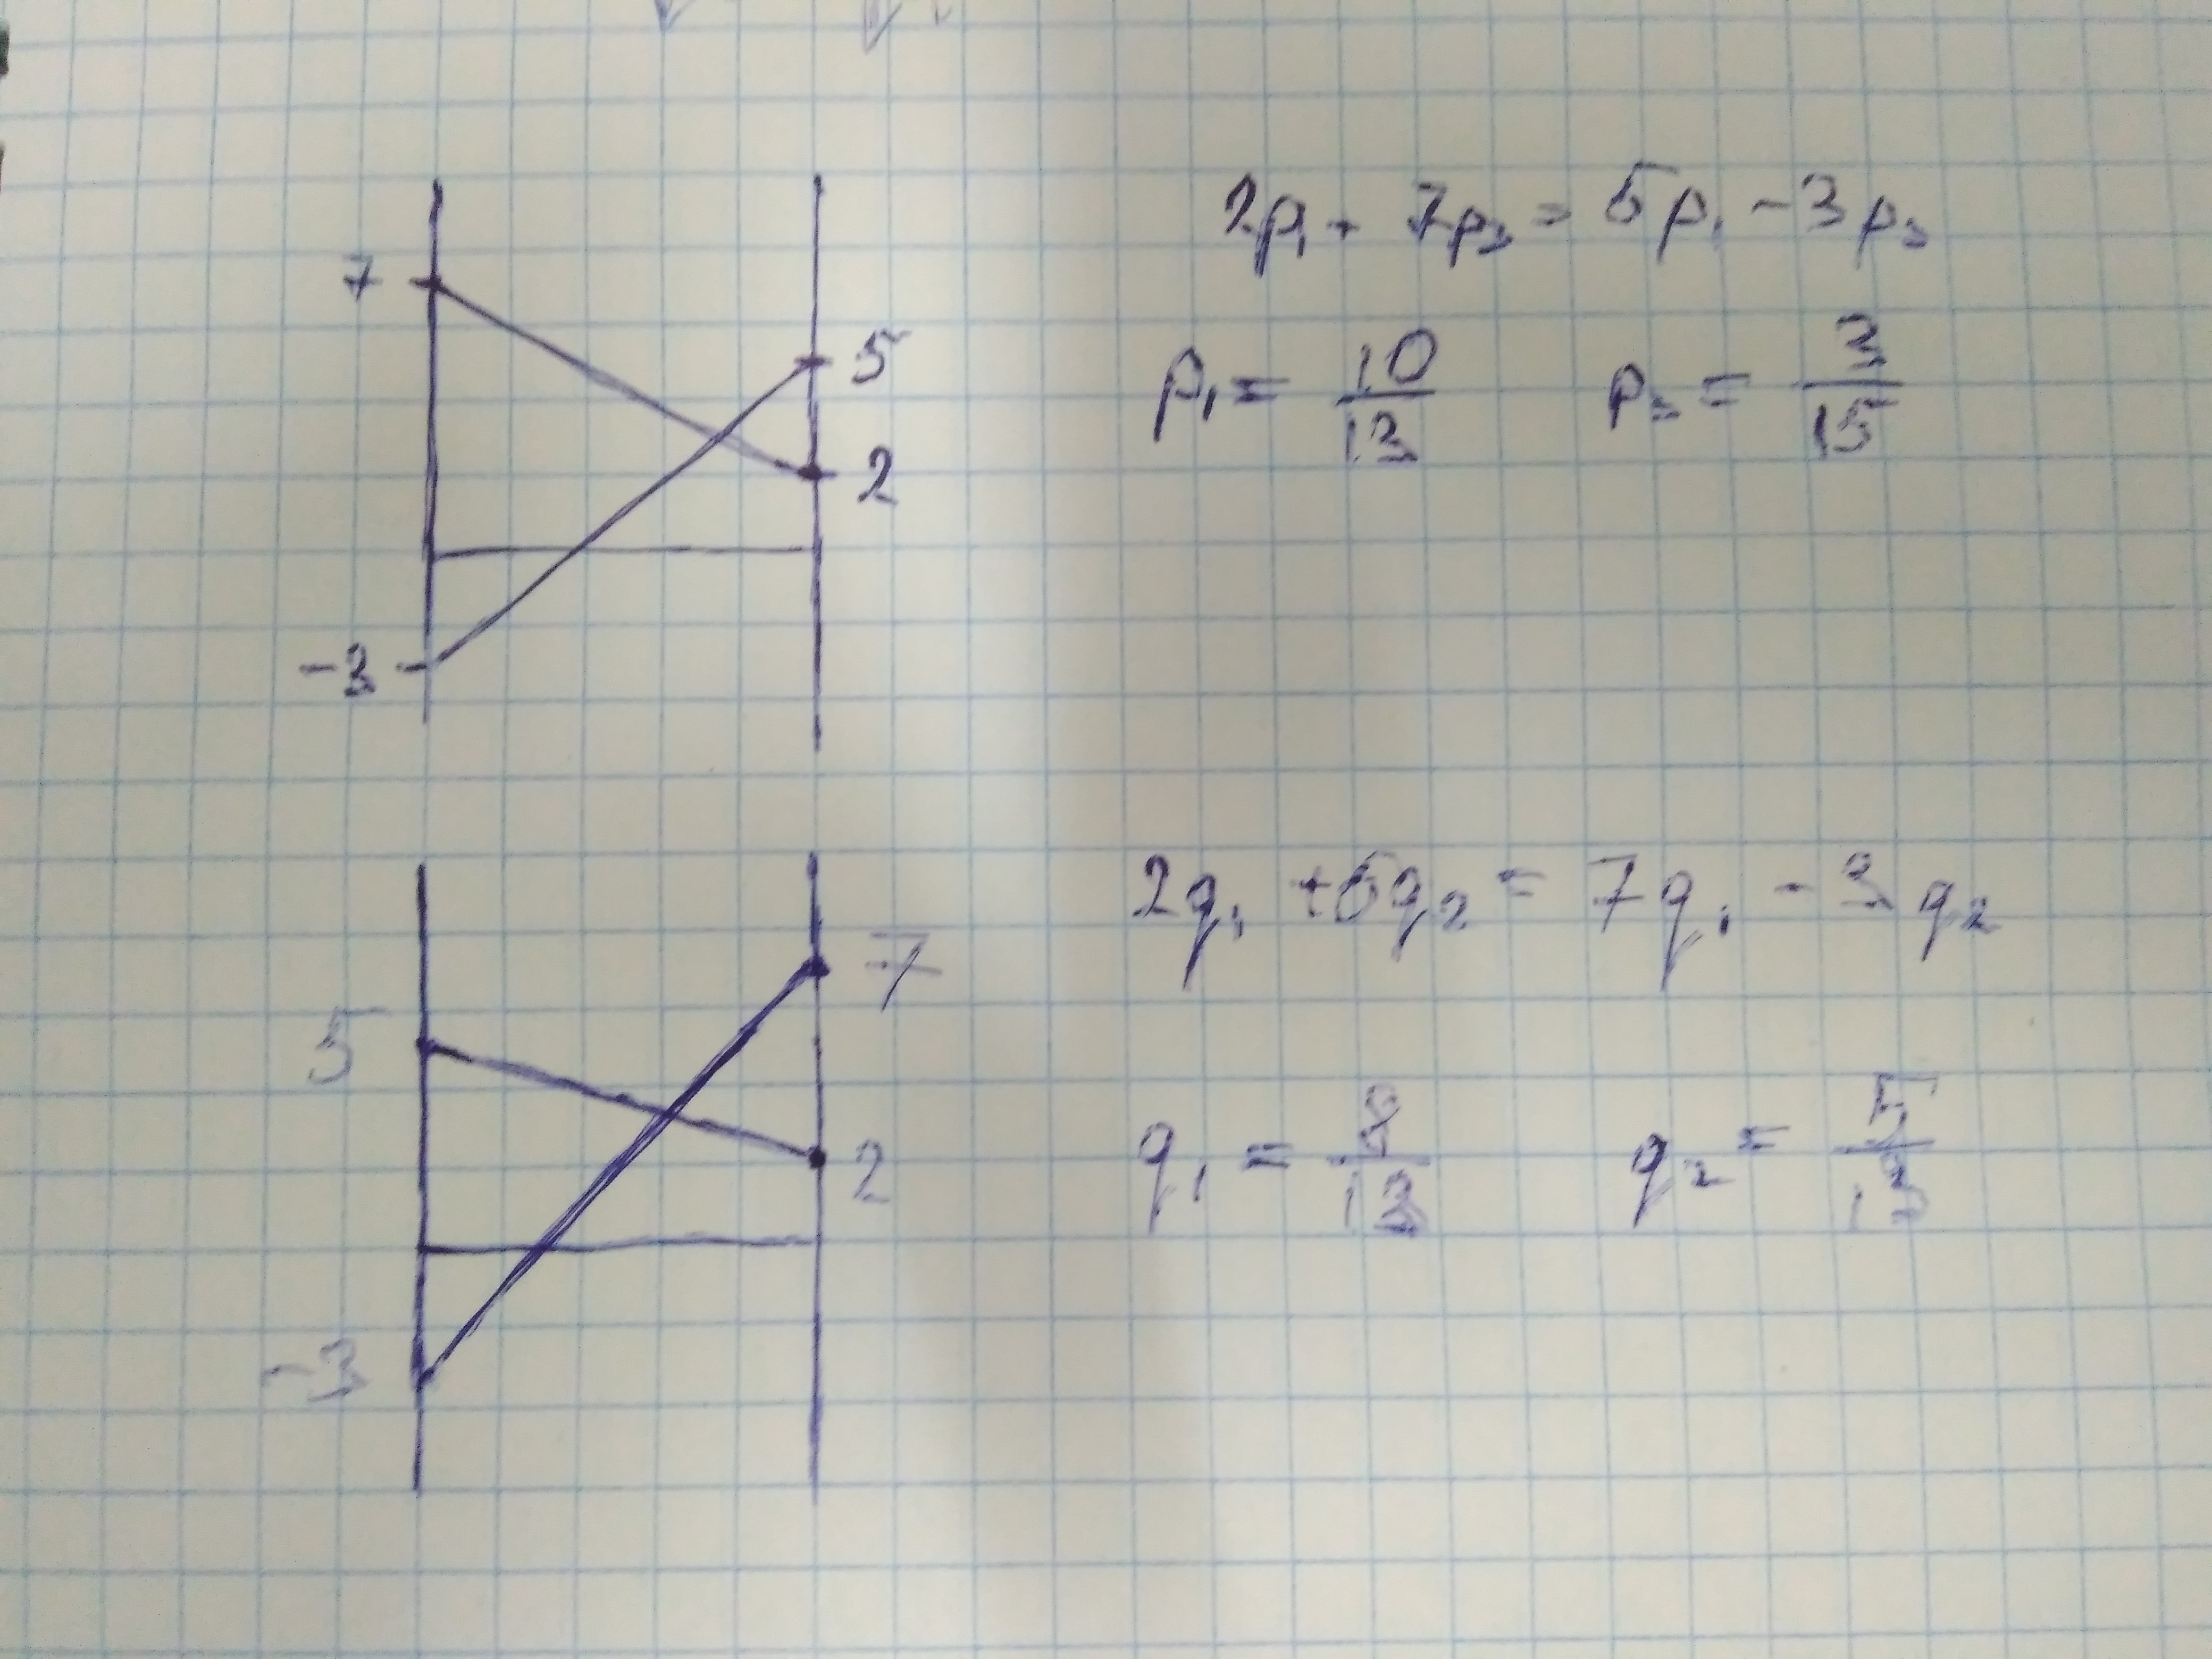
\includegraphics[scale=0.1]{IMG_20180406_001049.jpg}
\begin{gather*}
I = \frac{5}{7}
\end{gather*}
\subsection*{11a}
Показать, что если $h_{i-1,j} - 2 h_{ij} + h_{i+1,j} \leq 0, i = \overline{2, n-1},
j = \overline{1, m} $, то в игре с матрицей $H = (h_{ij})_{n \times m}$ каждый игрок имеет оптимальную стратегию, в которой используется не более двух чистых стратегий;
\\
Решение:\\
Из условия задачи: $(h_{i-1,j}-h_{ij})+(h_{i+1,j}-h_{ij}) \leq 0$. Возможны два варианта. Либо $(h_{i + 1, j}-h_{ij})\leq0$, то есть $i$-ая строка доминирует $(i+1)$-ую и тогда $p_{i+1} = 0, i=\overline{2, n-1}, j=\overline{1, m}$. Либо $(h_{i-1,j}-h_{ij})\leq 0$, то есть i-ая строка доминирует (i-1)-ую и тогда $p_{i-1} = 0, i=\overline{2, n-1}, j=\overline{1, m}$. В обоих случаях матрица выигрышей сокращается до размеров $2\times 2$. Затем можно найти оптимальные стратегии игроков, а так как матрица имеет размеры $2\times 2$, то у каждого игрока для оптимальной стратегии не более двух чистых стратегий.
\subsection*{11b}
Показать, что если $h_{i-1,j} - 2 h_{ij} + h_{i+1,j} \geq 0, i=\overline{2, n-1}, i=\overline{1, m}$, то в игре с матрицей $H=(h_{ij})_{n \times m}$ первый игрок имеет оптимальную стратегию $p$, для которой $p_i = 0, i=\overline{2, n-1}$.\\
Решение:\\
Из условия задачи: $(h_{i-1,j}-h_{ij})+(h_{i+1,j}-h_{ij})\geq 0$. Возможны два варианта. Либо $(h_{i+1,j}-h_{ij})$, то есть (i+1)-ая строка доминирует i-ую и тогда $p_i = 0, i=\overline{2, n-1}, j=\overline{1, m}$. Либо $(h_{i-1,j}-h_{ij})\geq 0$, то есть (i-1)-ая строка доминирует $i$-ую и тогда $p_i = 0, i=\overline{2, n-1}, j=\overline{1, m}$.
\section*{Матричные игры. Метод приближенных итераций}
\subsection*{12b}
\begin{gather*}H = \left(\begin{matrix}
1 & 0 & 4 & 7\\
3 & 5 & 2 & 0\\
0 & 1 & 3 & 5
\end{matrix}\right)\end{gather*}
Решение:\\
Верхнее значение игры $\beta=5$, нижнее $\alpha=0$. Решения в чистых стратегиях нет. Доминирования по строкам и столбцам нет.\\
\begin{tabular}{||c||c||c|c|c|c||c||c|c|c||c||c||c||}
\hline
k & i & $B_1$ & $B_2$ & $B_3$ & $B_4$ & $j$ & $A_1$ & $A_2$ & $A_3$ & $\underline{I}$ & $\overline{I}$ & $I$\\
\hline
1 & 1 & 1 & $\underline{0}$ & 4 & 7 & 2 & 0 & $\overline{5}$ & 1 & 0 & 5 & 2.5\\
\hline
2 & 2 & $\underline{2}$ & 2.5 & 3 & 3.5 & 1 & 0.5 & $\overline{4}$ & 0.5 & 2 & 4 & 3\\
\hline
3 & 2 & $\underline{2.33}$ & 3.33 & 2.67 & $\underline{2.33}$ & 1 & 0.67 & $\overline{3.67}$ & 0.33 & 2.33 & 3.67 & 3\\
\hline
4 & 2 & 2.5 & 3.75 & 2.5 & $\underline{1.75}$ & 4 & 2.25 & $\overline{2.75}$ & 1.5 & 1.75 & 2.75 & 2.25\\
\hline
5 & 2 & 2.8 & 5 & 2.4 & $\underline{1.4}$ & 4 & $\overline{3.2}$ & 2.2 & 2.2 & 1.4 & 3.2 & 2.3\\
\hline
\end{tabular}
\begin{gather*}
p_1 \approx \frac{1}{5}\\
p_2 \approx \frac{4}{5}\\
p_3 \approx 0\\
q_1 \approx \frac{2}{5}\\
q_2 \approx \frac{1}{5}\\
q_3 \approx 0\\
q_4 \approx \frac{2}{5}\\
I \approx \frac{23}{10}
\end{gather*}
\subsection*{12c}
\begin{gather*}H = \left(\begin{matrix}
2 & 3 & 1 & 0\\
0 & 2 & 4 & 2\\
3 & 0 & 1 & 2\\
4 & 1 & 0 & 1
\end{matrix}\right)\end{gather*}
Решение:\\
Верхнее значение игры $\beta=2$, нижнее $\alpha=0$. Решения в чистых стратегиях нет. Доминирования по строкам и столбцам нет.\\
\begin{tabular}{||c||c||c|c|c|c||c||c|c|c|c||c||c||c||}
\hline
k & i & $B_1$ & $B_2$ & $B_3$ & $B_4$ & $j$ & $A_1$ & $A_2$ & $A_3$ & $A_4$ &$\underline{I}$ & $\overline{I}$ & $I$\\
\hline
1 & 1 & 2 & 3 & 1 & $\underline{0}$ & 4 & 0 & $\overline{2}$ & $\overline{2}$ & 1 & 0 & 2 & 1\\
\hline
2 & 2 & $\underline{1}$ & 2.5 & 2.5 & $\underline{1}$ & 1 & 1 & 1 & $\overline{2.5}$ & $\overline{2.5}$ & 1 & 2.5 & 1.75\\
\hline
3 & 3 & 1.67 & 1.67 & 2 & $\underline{1.33}$ & 4 & 0.67 & 1.33 & $\overline{2.33}$ & 2 & 1.33 & 2.33 & 1.73\\
\hline
4 & 3 & 2 & $\underline{1.25}$ & 1.75 & 1.5 & 2 & 1.25 & 1.5 & $\overline{1.75}$ & $\overline{1.75}$ & 1.25 & 1.75 & 1.5\\
\hline
5 & 3 & 2.2 & $\underline{1}$ & 1.6 & 1.6 & 2 & $\overline{1.6}$ & $\overline{1.6}$ & 1.4 & $\overline{1.6}$ & 1 & 1.6 & 1.3\\
\hline
\end{tabular}
\begin{gather*}
p_1 \approx \frac{1}{5}\\
p_2 \approx \frac{1}{5}\\
p_3 \approx \frac{3}{5}\\
p_4 \approx 0\\
q_1 \approx \frac{1}{5}\\
q_2 \approx \frac{2}{5}\\
q_3 \approx 0\\
q_4 \approx \frac{2}{5}\\
I \approx \frac{13}{10}
\end{gather*}
\subsection*{12d}
\begin{gather*}H = \left(\begin{matrix}
2 & 4 & 5 & 1 & 5\\
1 & 5 & 0 & 6 & 2\\
3 & 0 & 2 & 1 & 1\\
1 & 2 & 1 & 0 & 3\\
\end{matrix}\right)\end{gather*}
Решение:\\
Верхнее значение игры $\beta=6$, нижнее $\alpha=1$. Решения в чистых стратегиях нет. Стратегия $A_1$ доминирует над стратегией $A_4$, $p_4 = 0$. Получаем сокращенную матрицу:\\
\begin{gather*}H = \left(\begin{matrix}
2 & 4 & 5 & 1 & 5\\
1 & 5 & 0 & 6 & 2\\
3 & 0 & 2 & 1 & 1\\
\end{matrix}\right)\end{gather*}
\begin{tabular}{||c||c||c|c|c|c|c||c||c|c|c||c||c||c||}
\hline
k & i & $B_1$ & $B_2$ & $B_3$ & $B_4$ & $B_5$ & $j$ & $A_1$ & $A_2$ & $A_3$ &$\underline{I}$ & $\overline{I}$ & $I$\\
\hline
1 & 1 & 2 & 4 & 5 & $\underline{1}$ & 5 & 4 & 1 & $\overline{6}$ & 1 & 1 & 6 & 3.5\\
\hline
2 & 2 & $\underline{1.5}$ & 4.5 & 2.5 & 3.5 & 3.5 & 1 & 1.5 & $\overline{3.5}$ & 2 & 1.5 & 3.5 & 2.5\\
\hline
3 & 2 & $\underline{1.33}$ & 4.67 & 2.67 & 4.33 & 3 & 1 & 1.67 & $\overline{2.67}$ & 2.33 & 1.33 & 2.67 & 2\\
\hline
4 & 2 & $\underline{1.25}$ & 4.75 & $\underline{1.25}$ & 4.75 & 2.75 & 1 & 1.75 & 2.25 & $\overline{2.5}$ & 1.25 & 2.5 & 1.88\\
\hline
5 & 3 & 1.6 & 3.8 & $\underline{1.4}$ & 5 & 2.4 & 3 & $\overline{2.4}$ & 2.2 & 2.2 & 1.4 & 2.4 & 1.9\\
\hline
\end{tabular}
\begin{gather*}
p_1 \approx \frac{1}{5}\\
p_2 \approx \frac{3}{5}\\
p_3 \approx \frac{1}{5}\\
p_4 \approx 0\\
q_1 \approx \frac{3}{5}\\
q_2 \approx 0\\
q_3 \approx \frac{1}{5}\\
q_4 \approx \frac{1}{5}\\
q_5 \approx 0\\
I \approx \frac{19}{10}
\end{gather*}
\end{document}